\documentclass[jou,a4paper,notxfonts]{apa}
\usepackage{graphicx} 
\usepackage{palatino}
\usepackage{fancyhdr}
\pagestyle{fancy}

% header on first page
\fancypagestyle{plain}{%
\fancyhf{} % clear all header and footer fields
\fancyhead[L]{\small
Journal of Eye Movement Research\\
1(1):1, 1-2}
\fancyfoot[C]{\thepage}
\renewcommand{\headrulewidth}{0pt}
\renewcommand{\footrulewidth}{0pt}}

\title{Distributed Eye Tracking Network for Conveying Population Gaze in a Mobile Telepresence Scenario} %Fill this in

%please refer to http://www.ilsp.gr/homepages/protopapas/apacls.html#titlhead for different numbers of authors and affiliations
\threeauthors{First Author}{Second Author}{Third Author}
\threeaffiliations{First affiliation}{Second Affiliation}{Third Affiliation}


\journal{}
\volume{}

\abstract{Mobile telepresence technology allows one or several remote users to visit a distant geographical space using
a mobile robot. The robot can carry a 360$^\circ$ panoramic camera that provides an immersive viewing environment to the
remote users of the robot location. One limitation of this technology is that for humans around the robot or elsewhere,
is difficult to gather a sense of where in the robot's location the remote users are paying attention to. Here, we
propose the usage of a distributed network of low cost eye trackers to monitor the gaze behavior and field of view
within the panoramic video of several remote users using a telepresence system. We transmit the gaze gaze behavior of
the remote users to the robot that then superimposes the aggregated gaze behavior of the remote users in a condensed 2D
representation of the panoramic image it is currently capturing. We use as an illustrative application, a robot being
employed to visit a museum virtually by several high school students in remote locations. A human  museum guide, directs
the robot around the museum while explaining and interacting with the remote students through the visual display on the
robot. The visual display of the robot can show a 2 dimensional condensed representation of the panoramic image being
captured by the robot with the superimposed gaze behavior data of the remote students. This visualization provides a
useful feedback signal to the tour guide about where the remote students are paying attention to so he can adapt his
behavior accordingly.

\linebreak
\linebreak
{\bf Keywords: keyword, keyword}}

\acknowledgements{}
\shorttitle{}
\rightheader{}

% repeat the authors here (use et al if more than three authors):
\leftheader{ }

\begin{document}

%-------------------------------------
\maketitle


\lhead{\small
Journal of Eye Movement Research\\
1(1):1, 1-2
}
\rhead{
Author, A., Author, B., & Author, C. (2007)\\
Short Title
}
\thispagestyle{plain}

\section{Introduction} 
Bla bla bla



\section{Method}

\subsubsection{Eye-tracking system}
Eyes are used by humans to obtain information about the surroundings and to communicate information. When something
attracts our attention, we position our gaze on it, thus performing a \textit{fixation}. A fixation usually has a
duration of at least 150 milliseconds (ms). The fast eye movements that occur between fixations are known as
\textit{saccades}, and they are used to reposition the eye so that the object of interest is projected onto the fovea.
The direction of gaze thus reflects the focus of \textit{attention} and also provides an indirect hint for
\textit{intention} \cite{velichkovsky}.


A video-based gaze tracking system seeks to find where a person is looking, i.e. the Point of Regard (PoR), using images
obtained from the eye by one or more cameras. Most systems employ infrared illumination that is invisible to the human
eye and hence it is not distracting for the user. Infrared light improves image contrast and produces a reflection on
the cornea, known as corneal reflection or glint. Eye features such as the corneal reflections and the center of the
pupil/iris can be used to estimate the PoR. Figure \ref{screenGazeTracker} shows a screenshot of an eye being tracked by
the open-source ITU Gaze Tracker \cite{lowcostitugazetracker,Rozado2012}. In this case, the center of the pupil and two
corneal reflections are the features being tracked.


\begin{figure}[tp]
 %\fitbitmap[scale=0.5]{figures/screenGazeTracker.jpg}
 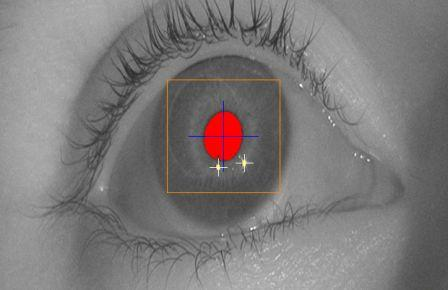
\includegraphics[width=0.5\textwidth, height=40mm]{figures/screenGazeTracker.jpg}
 \caption{\textbf{The Open Source ITU Gaze Tracker Tracking One Eye.} The
  features tracked in the image are the pupil center and two corneal reflections. These features are used by the gaze 
  estimation algorithms to determinine the PoR of the user on the screen.}
 \label{screenGazeTracker}
\end{figure}


\subsection{Apparatus}

\begin{figure}[tp]
 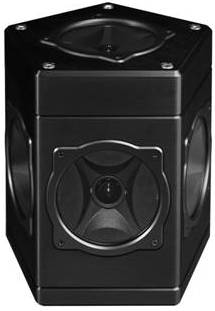
\includegraphics[width=0.3\textwidth, height=60mm]{figures/ladybug.jpg}
 %\fitbitmap{figures/ladybug.jpg}
 \caption{An image displaying the 360 degree panoramic camera on top of the robot}
 \label{ladybug}
\end{figure}

\begin{figure}[tp]
 \fitbitmap{figures/museumtourview.jpg}
 \caption{Remote interface client through which student can look around the
museum with freedom to look at different areas within the 360 field of view environment}
 \label{museumtourview}
\end{figure}

\begin{figure}[tp]
 \fitbitmap{figures/aggregatedGazeBehavior.jpg}
 \caption{Network of eye trackers on the remote students computer captures the gaze behavior of the students and
 combines the gaze data into a high-resolution omni-directional image}
 \label{aggregatedGazeBehavior}
\end{figure}

\begin{figure}[tp]
 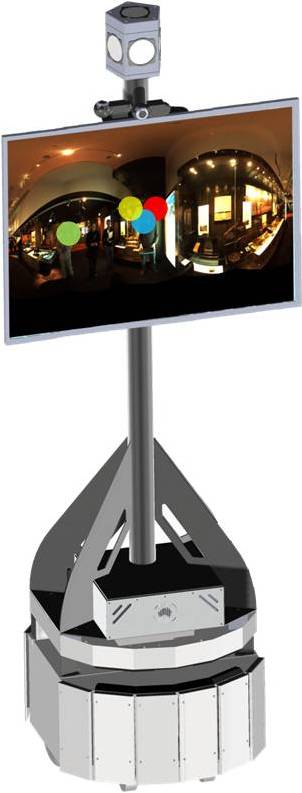
\includegraphics[width=0.4\textwidth, height=140mm]{figures/robotDisplay.jpg}
 \caption{Aggregated gaze behavior of remote
students superimposed into the omni-directional is shown in the robot display so the tour guide for instance can obtain
feedback about what areas in space the remote students are paying attention to}
 \label{robotDisplay}
\end{figure}


The telepresence robot carries a head-height omni-directional camera and a display screen, see
Figure \ref{ladybug}. It also has a forward-looking camera and a number of onboard computers and wifi antennas.

The educator wears a wireless lapel microphone, to ensure that he can be heard clearly by the remote students. They
can see who is online, and which students have questions via the display on the front of the robot.

The robot moves at walking speed within any wheelchair accessible space. It intelligently navigates to different
locations in the museum under the supervision of the educator or guide. It can sense walls, exhibits, and people around
it using a laser scanner. The robot�s navigation is based on a self-generated map of the gallery space and a
dynamic obstacle avoidance system.

Using a 360 degree camera mounted on top of the robot, a high resolution omni-directional image is constructed and
streamed. Each remote student can then independently �look around� the gallery using a panoramic viewer within their
browser, see Figure{museumtourview}.

Each student computer is equipped with a low cost eye tracker capturing frames at 30Hz. The students focus of attention
in the panoramic viewer is recorded. This includes the horizontal and vertical field of views (that determine the plane
being displayed on screen at any given time) and the x, y coordinate of their gaze on screen. This for parameters define
the point in 3D space the student is looking at. This aggregated data is sent back to the robot, that converts it to a
3D point in space.

Images from the 360 degree camera on top of the robot are combined to form a high-resolution omni-directional image,
see Figure \ref{ladybug}, and the points of regard of several students are projected into this image to provide feedback
to the educator about where the students are paying attention to in the scene, see Figure \ref{aggregatedGazeBehavior}
and \ref{robotDisplay}.


The user studies to be carried out in the future will involved students (ages 10-16) from several national high schools.
Their gaze will be monitored through a network of low cost Tobii Rex eye trackers. These eye trackers offer a
resolution of 30 samples per second and produce gaze estimation with an average accuracy of 0.5 degrees at 60
cm from the screen. 


The eye trackers are connected through a network. The TCP protocol is used to issue commands to the eye trackers
such as start calibration, calculate results from calibration, start tracking, stop tracking. Gaze estimation is
sent through the UDP protocol, since the system can afford to lose some packets. 

The krpano panoramic viewer is used by the students to freely move within the 360$^\circ$ video stream. Javascript
scripts are used to gathered the horizontal and vertical field of view coordinates of each student through the panoramic 
image.

%---------------------------------------------------------------
\section{Application}

Bla bla bla

\section{Discussion}
Bla bla bla


\bibliography{library}
\end{document}

